%%%%%%%%%%%%%%%%%%%%%%%%%%%%%%%%%%%%%%%%%%%%%%%%%%%%%%%%%%%%%%%%%%%%%%%%%%%%%%%

\chapter{APRESENTAÇÃO DOS RESULTADOS}
\label{chp:1}

A bateria de testes realizada neste projeto consistiu de seis execuções: duas para cada um dos três compiladores, sendo a primeira com e a segunda sem vetorização ativada durante a compilação (ver Tabela \ref{tab:2_flags} para detalhes das flags de compilação utilizadas em cada caso). Os resultados obtidos na bateria de testes são apresentados a seguir para os três compiladores testados: \texttt{ICC} (versão 19.1), \texttt{PGI} (versão 19.1) e \texttt{GCC} (versão 8.3).

\section{Tempos de cada execução}

A Tabela \ref{tab:a} exibe os tempos obtidos em dez dos 151 loops de teste (cinco primeiros e cinco últimos) durante as seis execuções da bateria de testes.

\begin{table}[H]
\center
\caption{Tempos de execução em segundos obtidos em dez dos 151 loops da bateria de testes (ver arquivo \textit{results1.xlsx} do repositório).} 
\begin{tabular}{@{}l l l l l l l l l l@{}}
\toprule
% & & \multicolumn{3}{@{}c@{}}{Exercício 1 -- \texttt{prog.c}} & & \multicolumn{3}{@{}c@{}}{Exercício 2 -- \texttt{prog2.c}}\\
%\cmidrule{3-5} \cmidrule{7-9}
 & & \multicolumn{8}{@{}c@{}}{Tempos de execução [s]} \\
 \cmidrule{3-10}
 & & \multicolumn{2}{@{}c@{}}{\texttt{ICC}} & & \multicolumn{2}{@{}c@{}}{\texttt{PGI}} & &  \multicolumn{2}{@{}c@{}}{\texttt{GCC}} \\
\cmidrule{3-4} \cmidrule{6-7} \cmidrule{9-10}
Loop & & Não-vet. & Vet.  & &  Não-vet. & Vet.  & &  Não-vet. & Vet. \\
\midrule
S000  & &    0.414  &   0.169  & &    0.360 &    0.338   & &   0.540 &    0.170 \\
S111  & &   0.274   &  0.269   & &   0.269  &   0.290    & &  0.286  &   0.252 \\
S1111 & &   0.566   &  0.371   & &   0.581  &   0.580    & &  0.680  &   0.339 \\
S112  & &   0.628   &  0.631   & &   0.295  &   0.334    & &  0.811  &   0.436 \\
S1112 & &   0.616   &  0.243   & &   0.232  &   0.267    & &   0.808 &    0.329 \\
\multicolumn{1}{c}{\vdots} & & \multicolumn{1}{c}{\vdots}  & \multicolumn{1}{c}{\vdots}   & & \multicolumn{1}{c}{\vdots} & \multicolumn{1}{c}{\vdots}     & & \multicolumn{1}{c}{\vdots} & \multicolumn{1}{c}{\vdots} \\
vpvpv  & &  1.150  &  0.627   & &   0.664  &  0.628   & &  1.257   &  0.684 \\
vtvtv  & &  1.156  &  0.630   & & 0.673   &  0.630    & &  1.268   &  0.685 \\
vsumr  & &  2.005  &  0.418   & &  4.006  &   0.502   & &   4.009  &   4.007 \\
vdotr  & &  2.055  &  0.904   & &  4.013  &   0.890   & &   4.013  &   4.010 \\
vbor   & &  0.133  &  0.089   & &  0.358  &   0.045   & &   0.358  &   0.090 \\
\bottomrule
\end{tabular}
\label{tab:a}
\end{table}

A Figura \ref{fig:a} exibe os histogramas dos tempos de execução obtidos com os três compiladores testados, para compilações sem vetorização (barras de cor laranja) e com vetorização (barras de cor azul). Os histogramas também apresentam as estatísticas de cada caso.

\begin{figure}[ht!]
	\vspace{0mm}	% acrescentar o espaçamento vertical apropriado entre o título e a borda superior da figura
	\begin{center}
		\resizebox{\textwidth}{!}{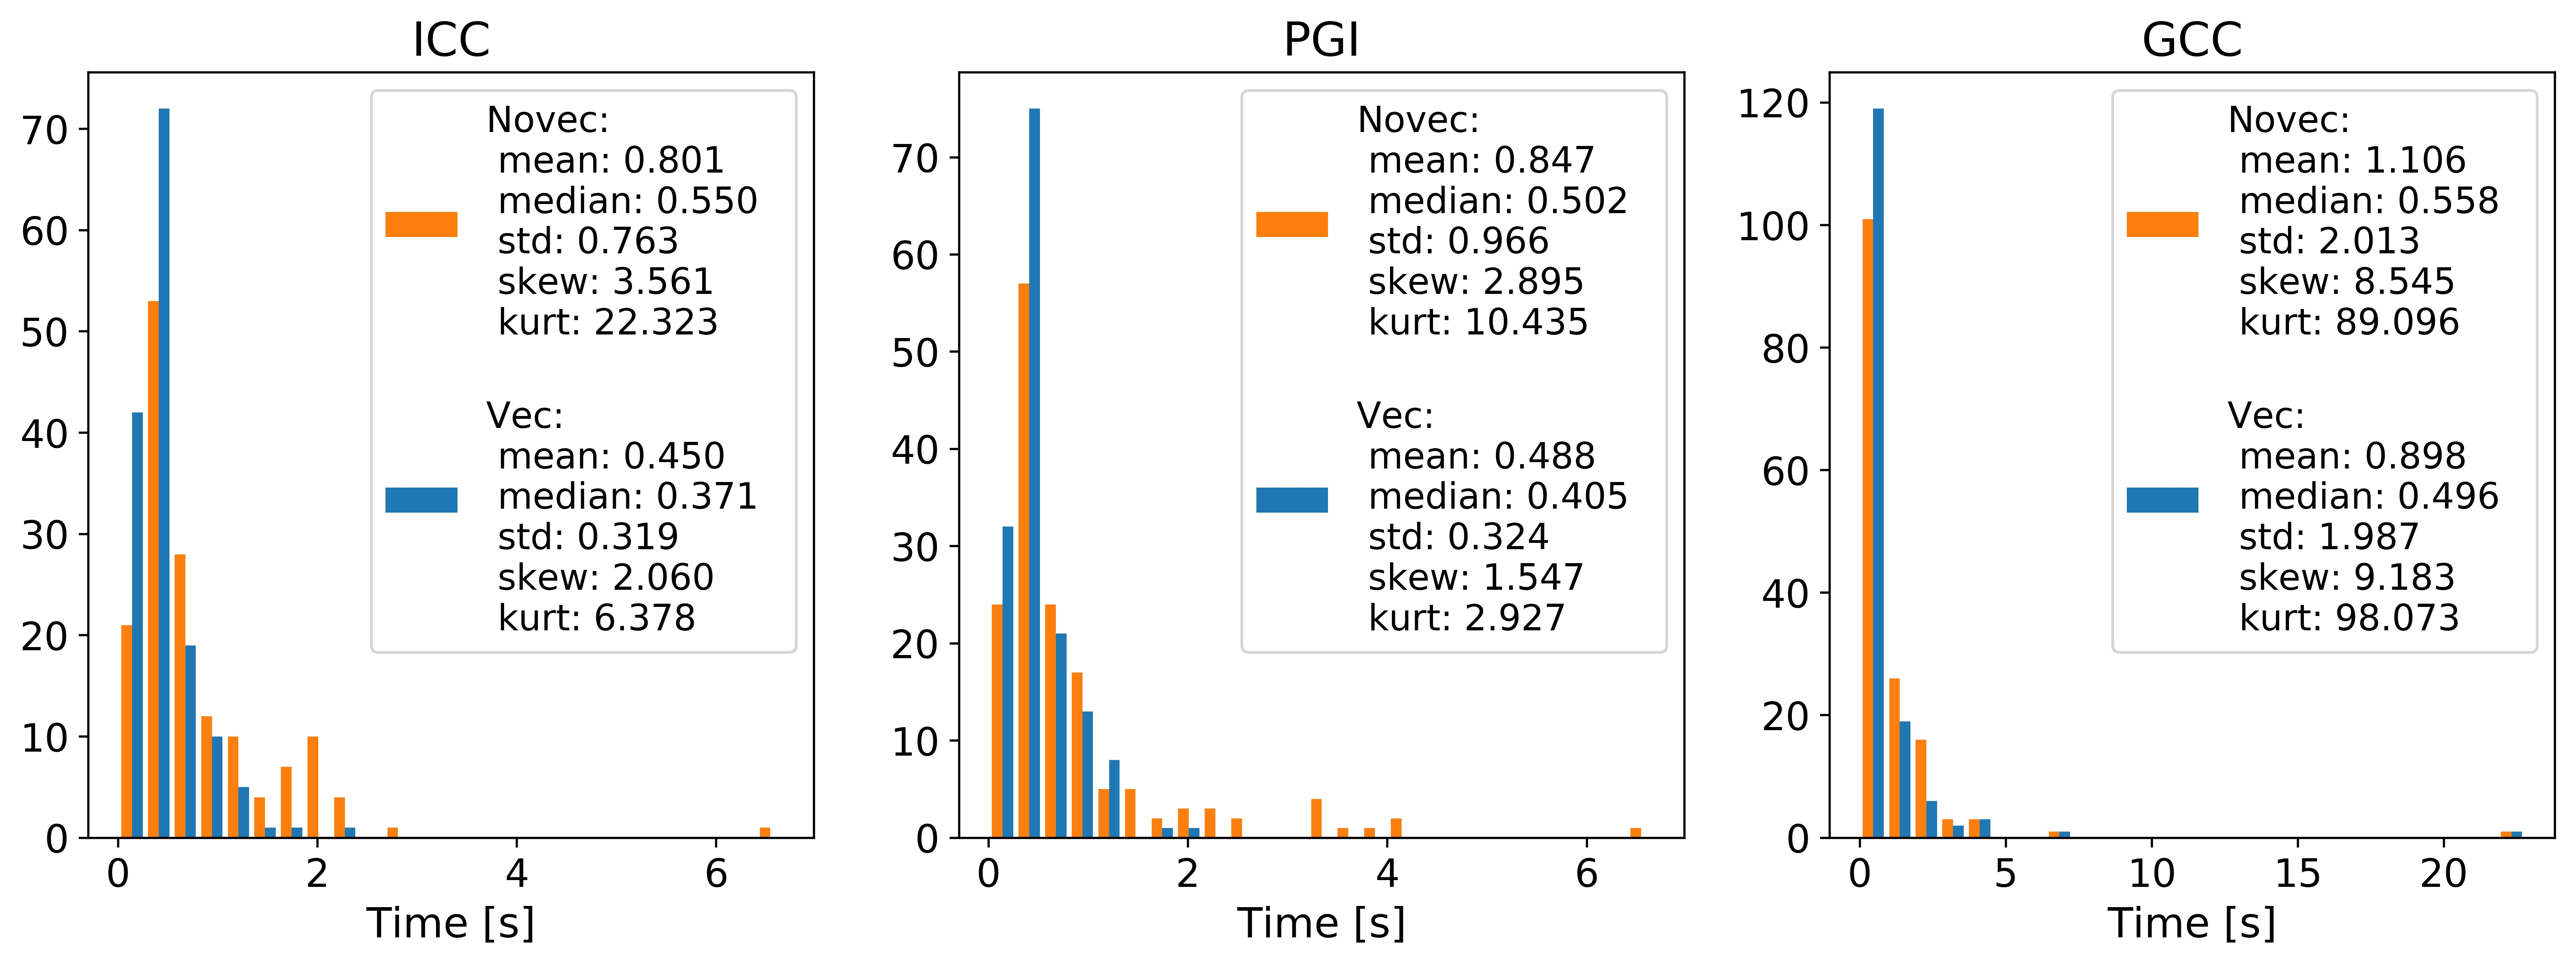
\includegraphics{Figuras/stats.jpg}}		
	\end{center}
	\vspace{2mm}	% acrescentar o espaçamento vertical apropriado entre a borda inferior da figura e a legenda ou a fonte quando não há legenda (o valor pode ser negativo para subir)
	\caption{Histogramas dos resultados obtidos nas execuções sem vetorização (barras de cor laranja) e com vetorização (barras de cor azul) dos três compiladores testados. O número de bins é igual a 25. As estatísticas de cada distribuição estão indicadas, incluindo a média (\textsf{mean}), mediana (\textsf{median}), o desvio padrão (\textsf{std}), o coeficiente de assimetria (\textsf{skew}) e o coeficiente de curtose (\textsf{kurt}).}
	\legenda{}	% legenda - para deixar sem legenda usar comando \legenda{} (nunca deve-se comentar o comando \legenda)
	\label{fig:a}
%	\FONTE{FOnte da imagem (se necessário).}	% fonte consultada (elemento obrigatório, mesmo que seja produção do próprio autor)
\end{figure}


\section{\textit{Speedups} de cada execução}

A Tabela \ref{tab:b} apresenta os \textit{Speedups} de dez dos 151 loops para os três compiladores testados, obtidos através da Tabela \ref{tab:a}.

\begin{table}[H]
\center
\caption{\textit{Speedups} de dez dos 151 loops da bateria de testes (ver arquivo \textit{results1.xlsx} do repositório).} 
\begin{tabular}{@{}l l l l l@{}}
\toprule
 & & \multicolumn{3}{@{}c@{}}{\textit{Speedups}}\\
 \cmidrule{3-5} 
Loop & & \texttt{ICC} & \texttt{PGI} &  \texttt{GCC} \\
\midrule
S000    & &   2.45    &   1.07   &   3.18 \\
S111    & &   1.02    &   0.93   &   1.13 \\
S1111   & &   1.53    &   1.00   &   2.01 \\
S112    & &   1.00    &   0.88   &   1.86 \\
S1112   & &   2.53    &   0.87   &   2.46 \\
\multicolumn{1}{c}{\vdots} & & \multicolumn{1}{c}{\vdots} & \multicolumn{1}{c}{\vdots} & \multicolumn{1}{c}{\vdots} \\
vpvpv    & &   1.83   &   1.06     &   1.84 \\
vtvtv    & &   1.83   &   1.07     &   1.85 \\
vsumr    & &   4.80   &   7.98     &   1.00 \\
vdotr    & &   2.27   &   4.51     &   1.00 \\
vbor     & &   1.49   &   7.96     &   3.98 \\
\bottomrule
\end{tabular}
\label{tab:b}
\end{table}


\section{\textit{Speedups} médios}

A partir da Tabela \ref{tab:b}, foi calculado o \textit{Speedup} médio de cada compilador:

\begin{table}[H]
\center
\caption{Médias dos 151 \textit{Speedups} resultantes dos testes dos três compiladores.} 
\begin{tabular}{@{}l l l l@{}}
\toprule
& \texttt{ICC} & \texttt{PGI} &  \texttt{GCC} \\
\midrule
\textit{Speedup} médio & 1.79 & 1.96 & 1.41 \\ 
\bottomrule
\end{tabular}
\label{tab:c}
\vspace{-3mm}
\end{table}

\section{Tempos totais}

A partir da Tabela \ref{tab:a}, foi calculado o tempo total de cada execução da bateria de testes:


\begin{table}[H]
\center
\caption{Somas dos tempos obtidos nos 151 loops das seis execuções.} 
\begin{tabular}{@{}l l l l l l l l l@{}}
\toprule
& \multicolumn{2}{@{}c@{}}{\texttt{ICC}} & & \multicolumn{2}{@{}c@{}}{\texttt{PGI}} & &  \multicolumn{2}{@{}c@{}}{\texttt{GCC}} \\
\cmidrule{2-3} \cmidrule{5-6} \cmidrule{8-9}
& Não-vet. & Vet.  & &  Não-vet. & Vet.  & &  Não-vet. & Vet. \\
\midrule
Tempo total [s] & 120.891 &  67.916 & & 127.894  &  73.688  & &  166.968  &  135.628 \\
\bottomrule
\end{tabular}
\label{tab:d}
\vspace{-3mm}
\end{table}

Com os valores da Tabela \ref{tab:d}, os \textit{Speedups} dos compiladores \texttt{ICC}, \texttt{PGI} e \texttt{GCC} são, respectivamente, 1.78, 1.74 e 1.23 (comparar com os valores da Tabela \ref{tab:c}).

\section{Número de loops vetorizados e não-vetorizados}

Através da Tabela \ref{tab:b}, e utilizando o limiar de 1.5 adotado em \citeonline{maleki2011evaluation}, foi obtido o número de loops vetorizados e não-vetorizados pelos três compiladores testados:


\begin{table}[H]
\center
\caption{Número de loops vetorizados e não-vetorizados (dentre os 151 loops de teste) por cada compilador.} 
\begin{tabular}{@{}l l l l l l l l@{}}
\toprule
\multicolumn{2}{@{}c@{}}{\texttt{ICC}} & & \multicolumn{2}{@{}c@{}}{\texttt{PGI}} & &  \multicolumn{2}{@{}c@{}}{\texttt{GCC}} \\
\cmidrule{1-2} \cmidrule{4-5} \cmidrule{7-8}
Não-vet. & Vet.  & &  Não-vet. & Vet.  & &  Não-vet. & Vet. \\
\midrule
57    &    94     &&     101     &    50     &&     108   & 43 \\
\bottomrule
\end{tabular}
\label{tab:e}
\end{table}


\section{Loops não-vetorizados}

Considerando o mesmo limiar de 1.5, foi determinado o número de loops não-vetorizados por nenhum dos três compiladores testados. Ao todo, 45 loops nunca foram vetorizados durante a bateria de testes. Tais loops são mostrados a seguir:

\begin{table}[H]
\center
\caption{Nomes dos loops que não foram vetorizados por nenhum compilador. O total é igual a 45.} 
\begin{tabular}{@{}l l l l l l l l l@{}}
\toprule
S111 & S1113 & S114 & S1115 & S118 & S123 & S126 & S141 & S161 \\
S162 & S171 & S172 & S232 & S1232 & S252 & S255 & S256 & S257 \\
S258 & S277 & S281 & S293 & S2101 & S2111 & S31111 & S3110 & S3112 \\
S321 & S322 & S323 & S332 & S341 & S342 & S343 & S353 & S481 \\
S482 & S491 & S4112 & S4113 & S4114 & S4115 & S4116 & vag & vas \\
\bottomrule
\end{tabular}
\label{tab:f}
\end{table}

A Figura \ref{fig:f} resume a distribuição de loops vetorizados e não-vetorizados pelos três compiladores ao longo dos testes.


\begin{figure}[ht!]
	\vspace{0mm}	% acrescentar o espaçamento vertical apropriado entre o título e a borda superior da figura
	\begin{center}
\begin{tikzpicture}

\draw \firstcircle (90:3.5) node[text=black] {GCC};

\draw   (90:2.1) node[text=black] {4};

\draw   (0:0) node[text=black] {10};

\draw   (145:1.7) node[text=black] {25};

\draw   (40:1.7) node[text=black] {4};

\draw \secondcircle (210:4.5) node [text=black,below left] {ICC};

\draw   (210:3) node[text=black] {27};

\draw   (270:1.8) node[text=black] {32};

\draw \thirdcircle (330:3.5) node [text=black,below right] {PGI};

\draw   (330:2.5) node[text=black] {4};

%\draw (-6.5,3.5) circle (1) node [text=black] {45};

\draw (-5.6,-4) rectangle (4.2,4.5);% node [text=black,above left] {Vetorizados};

\draw (-4,2.8) circle (1);% node [text=black,above left] {Não-vetorizados};

\draw (-3.9,4.1) node[text=black] {Não-vetorizados};

%\draw (-4.7,2.6) rectangle (-2.2,3.9) node [text=black,above left] {Não-vetorizados};

\draw (-4,2.8) node[text=black] {45};

\end{tikzpicture}	
	\end{center}
	\vspace{2mm}	% acrescentar o espaçamento vertical apropriado entre a borda inferior da figura e a legenda ou a fonte quando não há legenda (o valor pode ser negativo para subir)
	\caption{Diagrama de Venn do número de loops vetorizados e não-vetorizados pelos compiladores \texttt{ICC}, \texttt{PGI} e \texttt{GCC} ao longo dos testes realizados.}
	\legenda{}	% legenda - para deixar sem legenda usar comando \legenda{} (nunca deve-se comentar o comando \legenda)
	\label{fig:f}
%	\FONTE{FOnte da imagem (se necessário).}	% fonte consultada (elemento obrigatório, mesmo que seja produção do próprio autor)
\end{figure}



%Citação dentro de parênteses: \cite{press1989fast} % com parenteses

%Citação fora de parênteses (na linha): \citeonline{frick1998wavelet} % sem parenteses

